% Indicate the main file. Must go at the beginning of the file.
% !TEX root = ../main.tex

%%%%%%%%%%%%%%%%%%%%%%%%%%%%%%%%%%%%%%%%%%%%%%%%%%%%%%%%%%%%%%%%%%%%%%%%%%%%%%%%
% 04_results
%%%%%%%%%%%%%%%%%%%%%%%%%%%%%%%%%%%%%%%%%%%%%%%%%%%%%%%%%%%%%%%%%%%%%%%%%%%%%%%%

\section{Results}
\label{results}

    \subsection{Detection}

    - after detection how many sequences are excluded

    - how many images are left per label

    \subsection{Classification Performance}

    All classification models performed well on their respective test sets.
    The balanced accuracy scores for each model are presented in \autoref{tab:bal_acc_by_model}.
    Pretrained models consistently outperformed those trained from scratch, as shown in \autoref{fig:bal_acc_img} for the image level scores.
    Generally, smaller models achieved slightly higher scores than larger ones, although these differences remained within one standard deviation.
    In particular, the pretrained EfficientNet-B0 reached the highest balanced accuracy of \(0.992\pm0.004\).
    Applying sequence-level classification to the image-level predictions improved balanced accuracy for every model, but only by \(0.001\) to \(0.005\), which again falls within a single standard deviation.  


    %==== table: overview_dataset ====%
    \begin{table}[H]
\centering
\caption{Balanced accuracy of all models -- shown as mean ± standard deviation.}
\label{tab:bal_acc_by_model}
\begin{tabular}{l c r c c}
\toprule
Model & Pretrained & Params (M) & Image BA-Score & Sequence BA-Score \\
\midrule
efficientnet\_b0 & Yes & 4 & 0.9921 ± 0.004 & 0.9947 ± 0.002 \\
densenet169 & Yes & 12 & 0.9904 ± 0.004 & 0.9939 ± 0.002 \\
resnet50 & Yes & 23 & 0.9899 ± 0.004 & 0.9934 ± 0.002 \\
vit\_b\_16 & Yes & 85 & 0.9885 ± 0.005 & 0.9933 ± 0.002 \\
\midrule
efficientnet\_b0 & No & 4 & 0.9856 ± 0.005 & 0.9898 ± 0.003 \\
densenet169 & No & 12 & 0.9863 ± 0.006 & 0.9899 ± 0.002 \\
resnet50 & No & 23 & 0.9850 ± 0.004 & 0.9888 ± 0.003 \\
vit\_b\_16 & No & 85 & 0.9767 ± 0.006 & 0.9856 ± 0.004 \\
\bottomrule
\end{tabular}
\end{table}
    %=================================%

    \begin{figure}[ht]
    \centering
    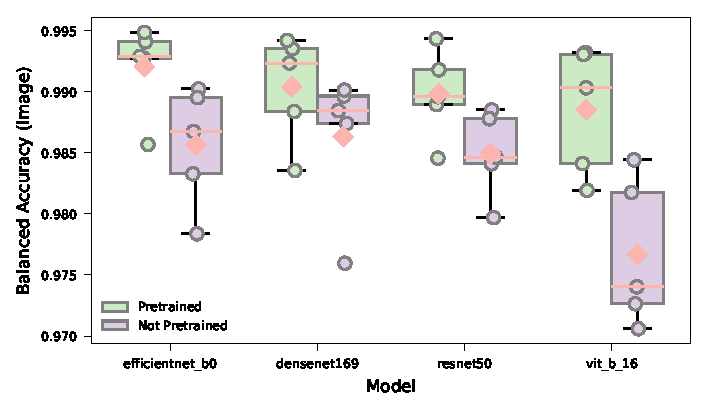
\includegraphics{figures/bal_acc_img.pdf}
    \caption{Balanced accuracy per model on the image level.}
    \label{fig:bal_acc_img}
    \end{figure}


    \subsection{Best Model}

    - More information on the best model including CM